\chapter{Hasil dan Pembahasan}

Bab ini menyajikan hasil pelaksanaan eksperimen dan pembahasannya. Seluruh angka berasal dari satu run bersih 50 epoch pada CPU dengan konfigurasi pada Tabel \ref{tab:konfigurasi}. Checkpoint, metrik, dan gambar disimpan pada direktori \texttt{outputs/} dan tidak disertakan dalam repositori karena berukuran besar.

\section{Dataset dan Distribusi Kelas}

Fashion-MNIST menyediakan 60.000 citra latih dengan distribusi kelas seimbang, yaitu 6.000 citra per kelas. Contoh satu citra per kelas ditunjukkan pada Gambar \ref{fig:samples-dataset} dan distribusinya pada Gambar \ref{fig:distribusi}. Keseimbangan ini menghindari bias kelas akibat jumlah sampel yang tidak merata, sehingga perbedaan kualitas antarkelas pada hasil generator lebih banyak dipengaruhi oleh kesamaan bentuk, bukan jumlah data.

\begin{figure}[H]
\centering
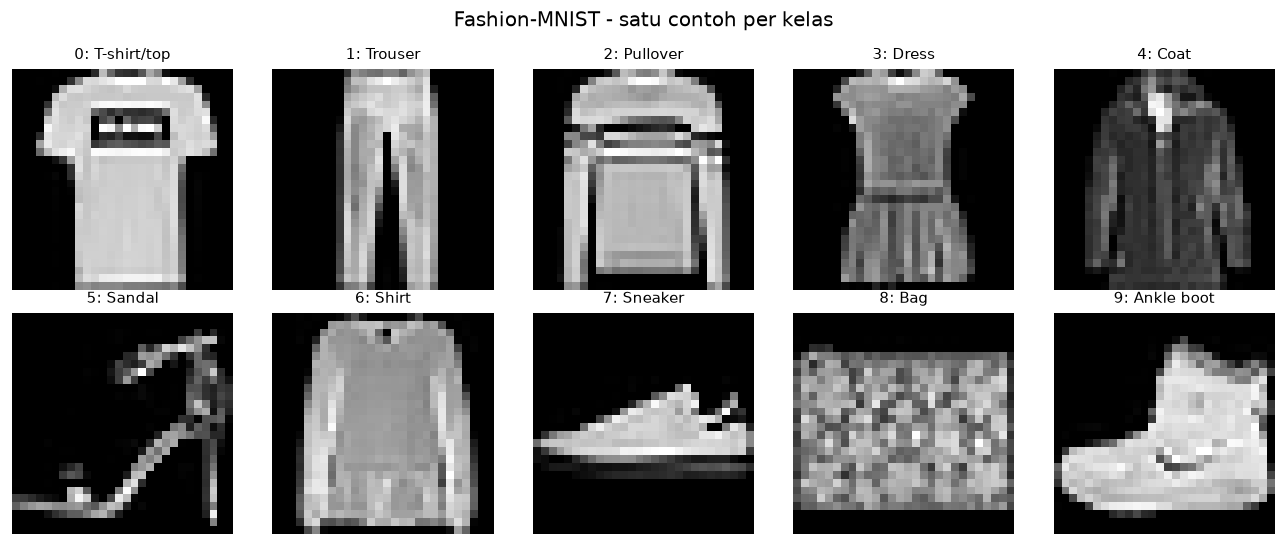
\includegraphics[width=0.92\textwidth]{dataset_samples.png}
\caption{Satu contoh citra asli untuk setiap kelas Fashion-MNIST}
\label{fig:samples-dataset}
\end{figure}

\begin{figure}[H]
\centering
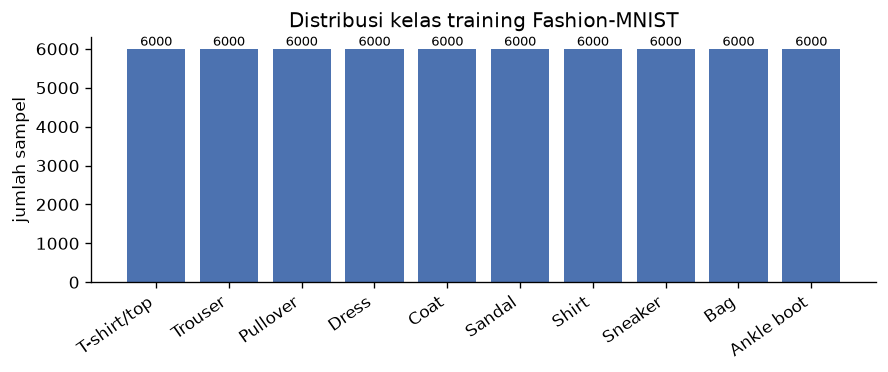
\includegraphics[width=0.85\textwidth]{class_distribution.png}
\caption{Distribusi jumlah sampel per kelas pada data latih}
\label{fig:distribusi}
\end{figure}

\section{Hasil Pelatihan}

Pelatihan 50 epoch selesai dalam 1.061,2 detik (\textit{wall-clock}) pada CPU tanpa percepatan perangkat keras khusus. Rata-rata loss pada beberapa epoch ditunjukkan pada Tabel \ref{tab:loss}. Nilai diambil dari epoch awal, tengah, dan akhir pelatihan.

\begin{table}[H]
\centering
\caption{Ringkasan loss pelatihan pada beberapa epoch}
\label{tab:loss}
\begin{tabular}{|L{1.5cm}|L{4.4cm}|L{4.4cm}|}
\hline
\textbf{Epoch} & \textbf{Loss Discriminator} & \textbf{Loss Generator} \\
\hline
1 & 0,3578 & 3,2119 \\
\hline
3 & 0,4285 & 3,6823 \\
\hline
25 & 1,1315 & 1,2639 \\
\hline
49 & 1,2561 & 0,9481 \\
\hline
50 & 1,2613 & 0,9564 \\
\hline
\end{tabular}
\end{table}

Kurva loss lengkap ditampilkan pada Gambar \ref{fig:loss}. Kedua kurva bergerak saling mendekat dan berosilasi di sekitar nilai 1 pada paruh kedua pelatihan. Pola ini menunjukkan permainan D dan G relatif seimbang, bukan berarti kualitas gambar terus meningkat, karena loss adversarial bersifat relatif terhadap kekuatan lawan.

\begin{figure}[H]
\centering
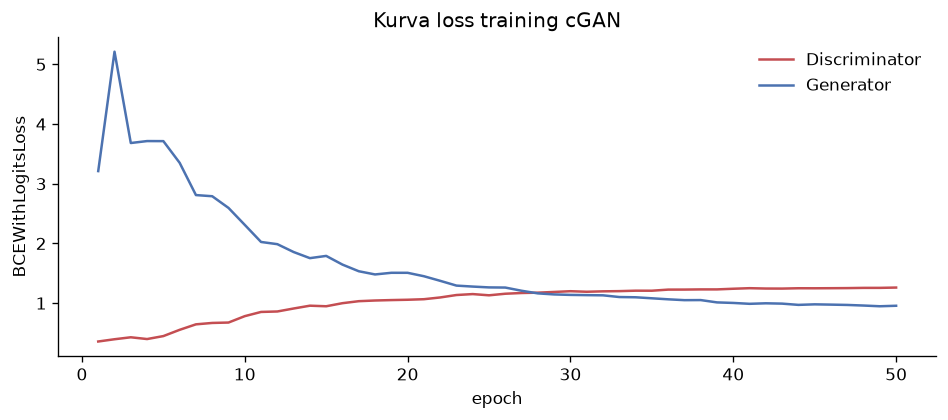
\includegraphics[width=0.88\textwidth]{loss_curve.png}
\caption{Kurva loss Discriminator dan Generator selama 50 epoch}
\label{fig:loss}
\end{figure}

\section{Pengaruh Jumlah Epoch terhadap Kualitas Visual}

Gambar \ref{fig:progresi} membandingkan keluaran tiga checkpoint berbeda menggunakan noise dan label yang sama. Perbandingan ini memberi gambaran langsung mengenai perkembangan bentuk, terlepas dari nilai loss. Pada epoch awal, citra masih berupa gumpalan abu-abu tanpa siluet yang jelas. Pada epoch pertengahan, bentuk kaus, tas, dan sepatu mulai muncul. Pada epoch akhir, kontras dan struktur siluet lebih tegas, meskipun masih terdapat kekaburan dan derau di latar.

\begin{figure}[H]
\centering
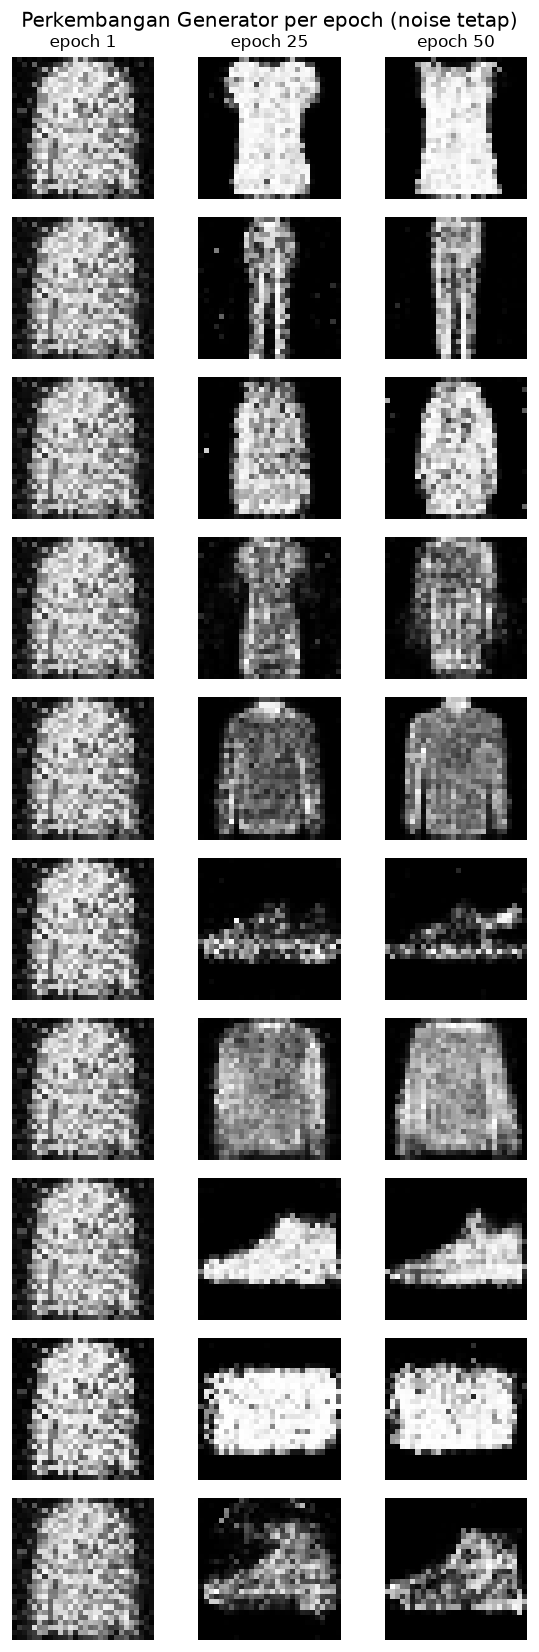
\includegraphics[height=0.82\textheight]{progression_by_epoch.png}
\caption{Perkembangan keluaran Generator pada epoch 1, 25, dan 50 dengan noise tetap}
\label{fig:progresi}
\end{figure}

\section{Sampel Hasil Generator}

Gambar \ref{fig:sampel-kelas} menyajikan empat sampel berbeda untuk setiap kelas dari checkpoint terakhir. Bentuk yang khas paling jelas terlihat pada kelas \textit{Trouser}, \textit{Bag}, \textit{Sneaker}, dan \textit{Ankle boot}. Sebaliknya, \textit{Shirt}, \textit{Pullover}, \textit{Coat}, dan \textit{Dress} cenderung saling menyerupai karena siluetnya beririsan.

\begin{figure}[H]
\centering
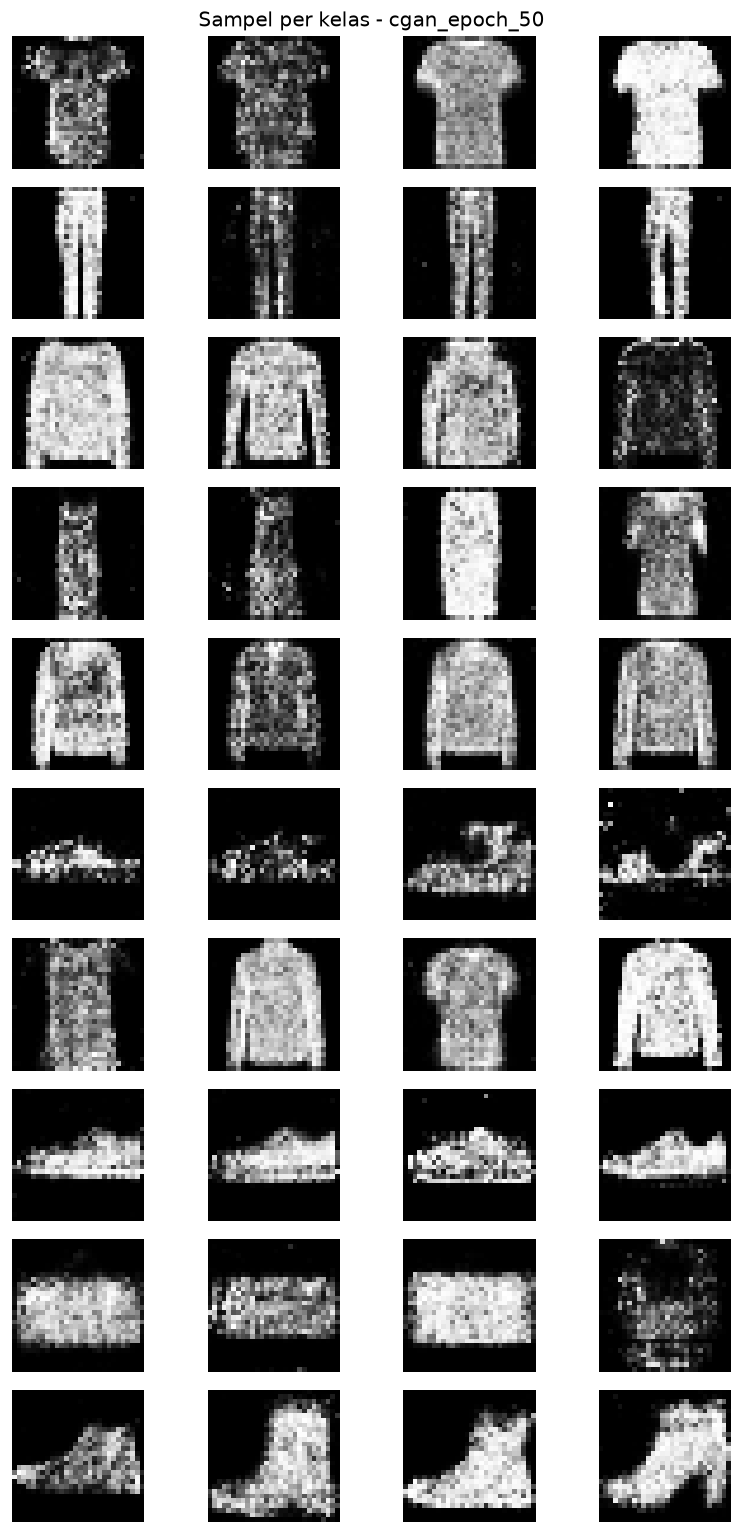
\includegraphics[height=0.86\textheight]{samples_per_class.png}
\caption{Empat sampel hasil Generator untuk setiap kelas pada epoch 50}
\label{fig:sampel-kelas}
\end{figure}

Grid satu gambar per kelas ditunjukkan pada Gambar \ref{fig:grid}. Bentuk grid ini dipakai untuk memeriksa secara cepat apakah \textit{conditioning} label bekerja, karena setiap kolom mewakili label berbeda dari satu vektor noise yang sama.

\begin{figure}[H]
\centering

\includegraphics[width=0.62\textwidth]{grid_one_per_class.png}
\caption{Grid satu sampel per kelas dari noise yang sama}
\label{fig:grid}
\end{figure}

\section{Keragaman Sampel}

Selain kesesuaian kelas, diperlukan pemeriksaan terhadap \textit{mode collapse}, yaitu kondisi ketika Generator menghasilkan variasi yang hampir sama untuk semua noise. Gambar \ref{fig:keragaman} menampilkan dua belas sampel per kelas untuk empat kelas representatif. Variasi bentuk masih terlihat, misalnya perbedaan kemiringan lengan pada kelas \textit{T-shirt} serta variasi sol pada \textit{Sneaker}. Dengan demikian, \textit{mode collapse} total tidak terjadi, meski variasi bentuknya tidak selebar data asli.

\begin{figure}[H]
\centering
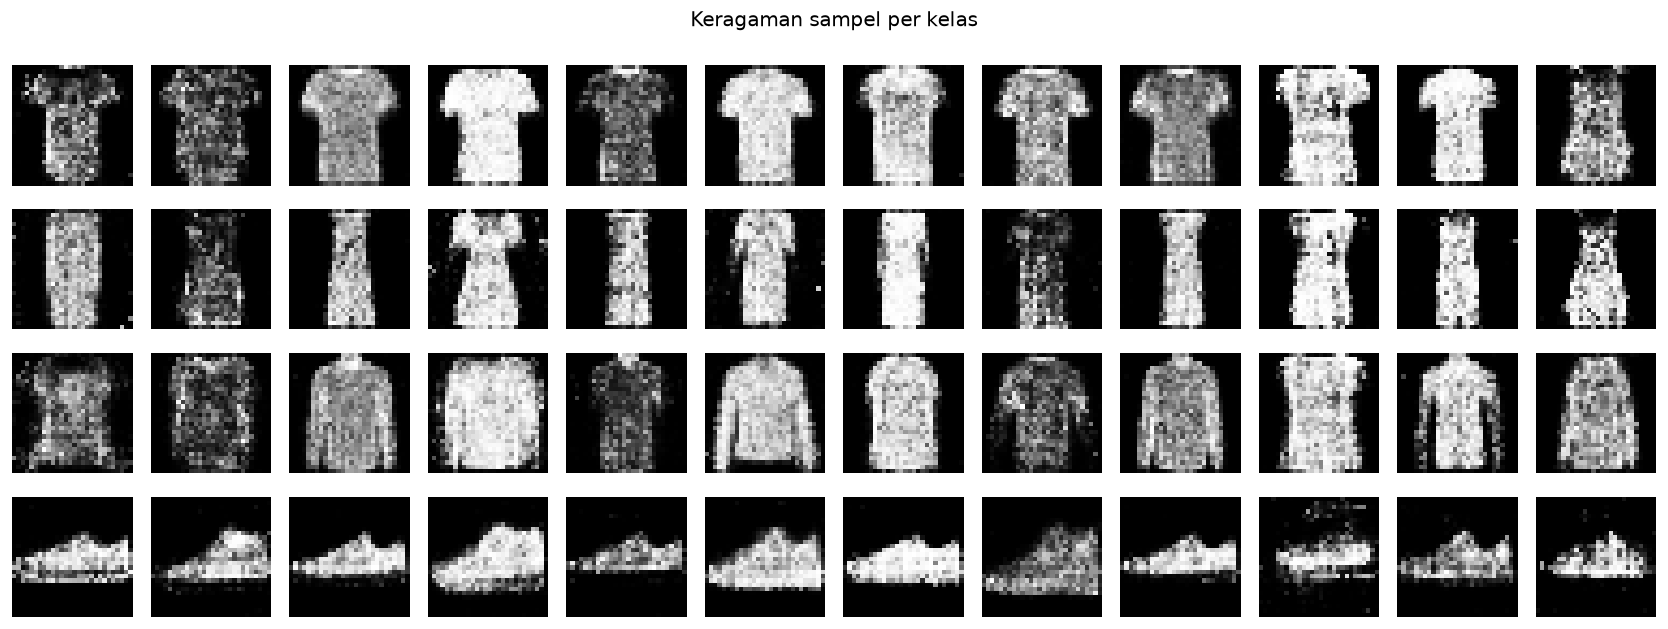
\includegraphics[width=\textwidth]{diversity_per_class.png}
\caption{Keragaman sampel dalam kelas yang sama (dua belas sampel)}
\label{fig:keragaman}
\end{figure}

\section{Hasil Evaluasi Kuantitatif}

Classifier MLP dilatih lima epoch pada data asli dan mencapai akurasi 0,8755 pada 10.000 citra uji. Angka ini menjadi pembanding untuk gambar generator. Hasil pada 100 gambar per kelas dirangkum pada Tabel \ref{tab:akurasi}.

\begin{table}[H]
\centering
\caption{Akurasi classifier pada gambar generator per kelas (100 sampel per kelas)}
\label{tab:akurasi}
\begin{tabular}{|L{1.1cm}|L{2.6cm}|L{1.9cm}|L{3.3cm}|}
\hline
\textbf{Label} & \textbf{Kelas} & \textbf{Akurasi} & \textbf{Keterangan} \\
\hline
0 & \textit{T-shirt/top} & 0,94 & tinggi \\
\hline
1 & \textit{Trouser} & 1,00 & tertinggi \\
\hline
2 & \textit{Pullover} & 0,84 & sedang \\
\hline
3 & \textit{Dress} & 0,89 & sedang \\
\hline
4 & \textit{Coat} & 0,75 & rendah \\
\hline
5 & \textit{Sandal} & 0,99 & tinggi \\
\hline
6 & \textit{Shirt} & 0,62 & terendah \\
\hline
7 & \textit{Sneaker} & 0,88 & sedang \\
\hline
8 & \textit{Bag} & 0,93 & tinggi \\
\hline
9 & \textit{Ankle boot} & 0,83 & sedang \\
\hline
\multicolumn{4}{|l|}{\textbf{Rata-rata} generator 0,8670 (asli 0,8755)} \\
\hline
\end{tabular}
\end{table}

Gambar \ref{fig:akurasi} memvisualkan perbandingan yang sama dalam bentuk diagram batang. Rata-rata akurasi generator 0,8670 hanya berselisih 0,0085 dari akurasi data asli. Selisih kecil ini perlu ditafsirkan hati-hati. Karena semua kelas pakaian berjumlah seimbang dan classifier cukup akurat, hasil ini menunjukkan bahwa mayoritas gambar generator sudah menyerupai kelas asalnya menurut pandangan classifier. Namun, classifier yang dipakai berkapasitas kecil sehingga belum tentu menangkap detail tekstur dan cacat lokal yang terlihat oleh mata manusia.

\begin{figure}[H]
\centering
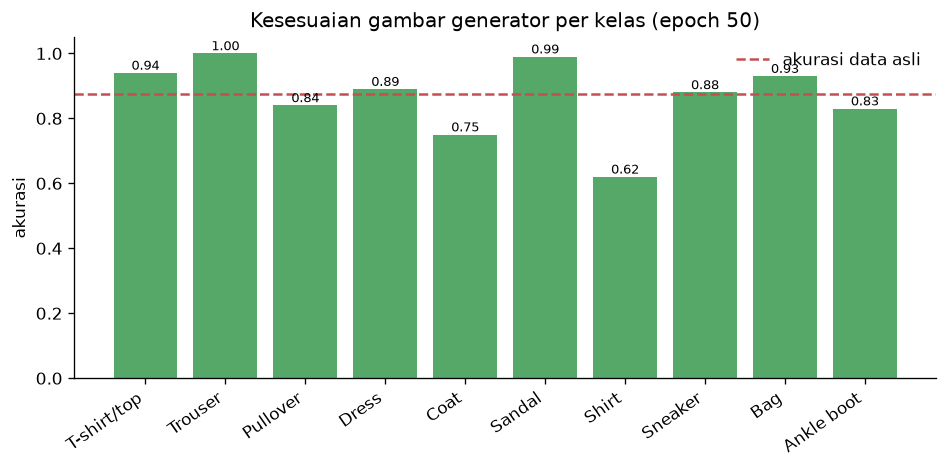
\includegraphics[width=0.88\textwidth]{classifier_accuracy.png}
\caption{Akurasi kesesuaian kelas gambar generator dengan garis pembanding akurasi data asli}
\label{fig:akurasi}
\end{figure}

\section{Pembahasan}

Tiga temuan utama dapat disimpulkan dari hasil di atas. Pertama, \textit{conditioning} label terbukti berpengaruh: gambar dengan label berbeda memiliki distribusi bentuk yang khas, dan kelas dengan siluet unik memperoleh akurasi tertinggi. Kedua, kelas yang secara visual mirip memperoleh akurasi terendah, yang konsisten dengan keterbatasan MLP dalam menangkap perbedaan halus seperti kerah dan panjang lengan. Ketiga, loss adversarial tidak sejalan lurus dengan kualitas visual; pada paruh kedua pelatihan, loss D justru naik sementara bentuk gambar membaik.

Perbandingan dengan arsitektur konvolusional menunjukkan bahwa DCGAN menghasilkan detail yang lebih tajam karena memanfaatkan struktur spasial \citep{radford2015dcgan}. Batasan ini sesuai dengan pilihan metodologis pada Bab III, dan perbaikan berupa lapisan konvolusi dapat diperlakukan sebagai eksperimen lanjutan terpisah tanpa mengubah kontrak data yang sudah ada.

Dari sisi rekayasa perangkat lunak, pemisahan modul menghasilkan pengujian yang dapat dijalankan cepat. Seluruh 36 pengujian lulus pada CPU dalam hitungan detik, termasuk pengujian bahwa perubahan label benar-benar memengaruhi keluaran Generator saat bobot dikendalikan, serta pengujian bahwa resume dari checkpoint melanjutkan penomoran epoch dengan benar.
